\chapter{Preliminaries}
\label{chapter:Prelims}

\section{Notation}

First we introduce notation for expressing graph metrics. This notation will also be used throughout the paper. % TODO - GET RID OF SECOND LINE?

\begin{definition}
	Complement Set

	\noindent
	Given a graph $G = (V, E)$, for a set of vertices $S \subseteq V$ we define the complement set $\comp{S} = V \setminus S$
\end{definition}

\begin{definition}
	Cut Set

	\noindent
	Given a graph $G = (V, E)$, for a set of vertices $S \subseteq V$ we define the cut set $ E(S, \comp{S}) = \left\{\{u, v\} \in E \mid u \in S, v \in \comp{S} \right\}.$
\end{definition}

\begin{definition}
	Degree of a vertex

	\noindent
	Given a graph $G = (V, E)$, let $d_v$ be the number of neighbouring nodes $v$ is adjacent to, i.e. $$
		d_v = |\left\{ e \in E : v \in e \right\}|
	$$
\end{definition}

\begin{definition}
	Volume of a vertex set

	\noindent
	Given a graph $G = (V, E)$ with $S \subseteq V$, let 
	$$
		\text{vol}(S) = \sum_{v \in S} d_v
	$$
\end{definition}

% TODO: Explain Implications of Cut set defn?

\section{Graph Metrics}\label{section:graphMetrics}

\begin{definition}
	Conductance of a graph $G = (V, E)$
	$$
		\Phi(G) = \min_{\emptyset \neq S \subset V} \frac{|E(S, \comp{S})|}{\min\{\text{vol}(S), \text{vol}(\comp{S})\}}
	$$
\end{definition}

\begin{definition}
	Diligence of a cut $ E(S, \comp{S}) $
	$$
		\rho(S) = \comp{d}(S) \min_{\{u, v\} \in E(S, \comp{S}) } \left\{ \max \left\{ \frac{1}{d_u},\frac{1}{d_v} \right\} \right\}
	$$ 
	where $\comp{d}(S) := \frac{\sum_{v \in S} d_v}{|S|}$ is the average degree of the vertices in $S$
\end{definition}

\begin{definition} % TODO: This definition doesn't include size bounds on S
	Diligence of a graph $G$
	$$
		\rho(G) = \min_{0 < \text{vol}(S) \leq \frac{\text{vol}(V)}{2}} \rho(S) 
	$$
\end{definition}

\section{Asymptotic Notation}

In this section, we review asymptotic notation for real valued functions. We assume the reader is familiar with this style of notation, but give precise definitions to avoid confusion. % TODO: Reword "avoid confusion"

The following definitions allow us to compare functions from the natural numbers to the reals.

\begin{definition}
	$\mathcal{O}$-Notation

	\noindent
	We say $f(n) = \mathcal{O}(g(n))$ if there exists a real constant $c > 0$ and $N \in \mathbb{N}$ such that $f(n) \leq c g(n)$ for all $n \geq N$. 
\end{definition}

\begin{definition}
	$\Omega$-Notation

	\noindent
	We say $f(n) = \Omega(g(n))$ if there exists a real constant $c > 0$ and $N \in \mathbb{N}$ such that $f(n) \geq c g(n)$ for all $n \geq N$. 
\end{definition}

\begin{definition}
	$\Theta$-Notation

	\noindent
	We say $f(n) = \Theta(g(n))$ if $f(n) = \mathcal{O}(g(n))$ and $f(n) = \Omega(g(n))$
\end{definition}


\begin{definition}
	$o$-Notation

	\noindent
	We say $f(n) = o(g(n))$ if for all $c > 0$, there exists $N \in \mathbb{N}$ such that $f(n) < c g(n)$ for all $n \geq N$.
\end{definition}

\section{Discrete-time Markov Chains}

In this section we give a brief review of Markov chains and associated results needed for Section \ref{section:MEDNBound}. We assume that the reader is familiar with finite Discrete-time Markov chains, so omit the proofs in this section. For a full treatment of the subject see \cite{grimmetBook}.

\begin{definition}
	Markov Chain

	\noindent A stochastic process $\{X_n, n \geq 0 \}$ on a state space $S$ is a Markov chain if 
	$$
		\mathbb{P}(X_n = s_n | X_0 = s_0, \dots,  X_{n-1} = s_{n-1}) 
		= \mathbb{P}(X_n = s_n | X_{n-1} = s_{n-1})
	$$
	for all $n \geq 1$ and $s_0, \dots, s_n \in S$.
\end{definition}

All the Markov chains we study in this section will operate on state spaces with a finite number of elements, so henceforth all results assume that the state space is finite. For simplicity, we also restrict our study to time homogenous Markov chains, that is Markov chains $\{X_n, n \geq 0 \}$ which satisfy
$$
	\mathbb{P}(X_{n+1} = i | X_n = j)
	= \mathbb{P}(X_1 = i | X_0 = j)
$$
for all $n \geq 1$ and $i, j \in S$.

\begin{definition}
	Transition Matrix

	The transition matrix of a Markov chain $\{X_n, n \geq 0 \}$ on a state space $S$ is an $|S| \times |S|$ matrix $P=(p_{ij})_{i, j \in S}$ such that
	$$
		p_{ij} = \mathbb{P}(X_1 = j | X_0 = i)
	$$
\end{definition}

\begin{definition}
	Stationary Distribution

	\noindent
	A row vector $\pi=(\pi_i)_{i \in S}$ is a stationary distribution of a Markov chain on a state space $S$ with transition matrix $P$ if
	\begin{enumerate}
		\item $p_i \geq 0$ for all $i \in S$
		\item $\sum_{i \in S} p_i = 1$
		\item $\pi P = \pi$
	\end{enumerate}
\end{definition}

\begin{definition}
	Irreducibility

	\noindent
	A Markov chain on a state space $S$ is irreducible if for all $i, j \in S$, there exists an $n \geq 0$ such that 
	$$
		\mathbb{P}(X_n = i | X_0 = j) > 0
	$$
\end{definition}

Intuitively, a Markov chain is irreducible if there is a non-zero probability of reaching any state after some finite number of time steps, regardless of which state the chain started in.

\begin{theorem}\label{theorem:uniqueStationaryDistribution}
	An irreducible Markov chain has a unique stationary distribution.
\end{theorem}

\begin{definition}
	Period

	\noindent
	The period of state $s \in S$ in a Markov chain $\{X_n, n \geq 0 \}$ is
	$$
		\gcd\{ n \geq 1 : \mathbb{P}(X_n = s | X_0 = s)\}
	$$
	If all states have period 1, we call the Markov chain aperiodic.
\end{definition}

% TODO: Intution - interested in how to prove??

\begin{theorem}\label{theorem:markovChainConvergence}
	If a Markov chain if irreducible and aperiodic, then the distribution of its current state after $n$ time steps converges to its stationary distribution as $n$ tends to infinity.
\end{theorem}

% TODO: Linking detail??

\section{Inhomogeneous Poisson Processes}\label{section:inhomoPP}

In this section we introduce an extension of the Poisson process which will be needed for the proof of Theorem \ref{theorem:AsyncUpperBound}.

\begin{definition}
	Counting Process

	\noindent
	A counting process $\left\{ N(t), t \geq 0 \right\}$ is a right-continuous non-decreasing random function $N$ from non-negative reals to non-negative integers such that $N(0) = 0$.
\end{definition}

\begin{figure}[h]
	\centering
	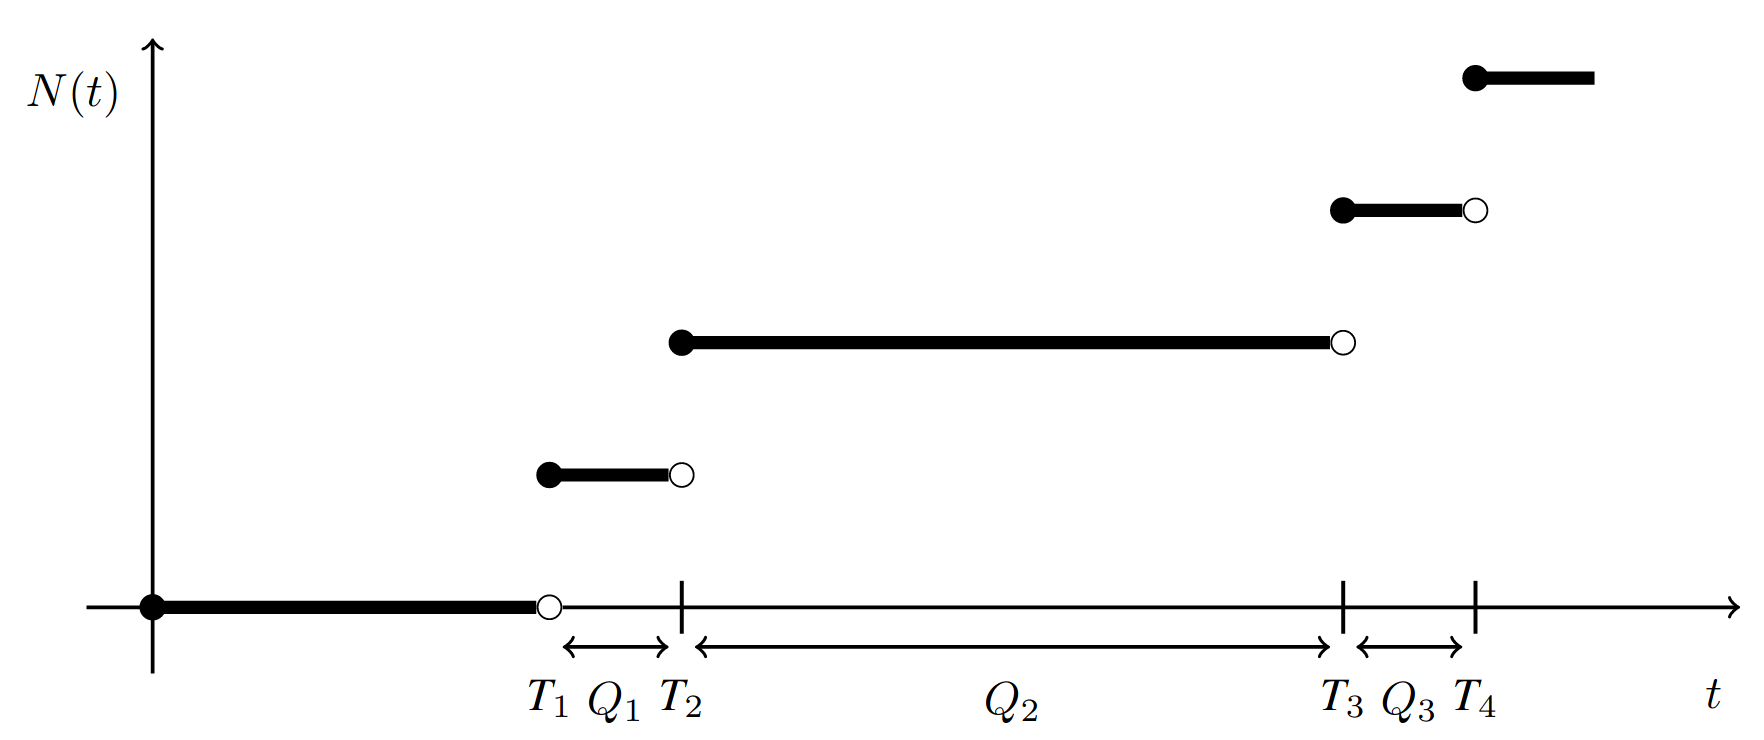
\includegraphics[width=\textwidth]{./figures/poisson_process_example.png}
	\caption{Example of a counting process from \cite{countingProcessFigure}}
	\label{fig:poissonProcessExample}
\end{figure}

% TODO: Discuss figure

We interpret the function $N$ as counting the number of occurrences of an event, where $N(t)$ represents the number of events that have occurred up to and including time $t$. We refer to the occurrences of events as "arrivals".  Since $N$ is right-continuous, $N$ increments exactly at the times of arrivals. For example, if $a^\text{th}$ arrival happens at time $t$, then $N(t) = a$, $\lim_{x \downarrow t} = a$, and $\lim_{x \uparrow t} = a - 1$. Note that the number arrivals in the interval $(s, t]$ is represented by the random variable $N(t) - N(s)$. 
%%% COUNTING PROCCESS END

\begin{definition}
	Inhomogeneous Poisson process

	\noindent
	An inhomogeneous Poisson process ${N(t), t \geq 0}$ with rate function $\lambda(t) > 0$ is a counting process such that
	\begin{enumerate}
		\item $N(t)$ has independent increments % TODO: What does this mean
		\item for all $0 \leq s \leq t$, 
		the number of arrivals in the interval $(s, t]$,  % TODO: Check this interval
		$N(t) - N(s)$, has a Poisson distribution with mean
		$$
			\Lambda(t) = \int_s^t \lambda(x) dx
		$$
		\item $N(0) = 0$
	\end{enumerate}
\end{definition}

In this process the rate of arrivals can vary over time. This property is reflected in part 2 of the definition ... % TODO: Finish

\begin{definition}
	Homogeneous Poisson Process

	\noindent
	A Homogeneous Poisson process ${N(t), t \geq 0}$ with rate $\lambda > 0$ is a special case of the inhomogeneous Poisson process where the rate function $\lambda(t)$ is constant i.e. $\lambda(t)=\lambda > 0$ for all $t$.
\end{definition}

% TODO: Reference superposition property + equivalence with exp arrival times

\section{Stochastic Domination}

% TODO: Intro

\begin{definition}
	First-order Stochastic Domination

	\noindent
	Let $X$ and $Y$ be real random variables. $Y$ has a first-order stochastic dominance over $X$, denoted by $X \preceq Y$, if for all $x \in R$, 
	$$
		\mathbb{P}(Y \geq x) \geq \mathbb{P}(X \geq x)
	$$
\end{definition}

Stochastic domination specifies a partial order between random variables. However, not all random variables are comparable by stochastic domination. % TODO: Exmaples

% TODO: interpretation as partial order and PDFs vs CDFS (gamma figure) 
% Not always the case

\begin{figure}[h]
	\centering
	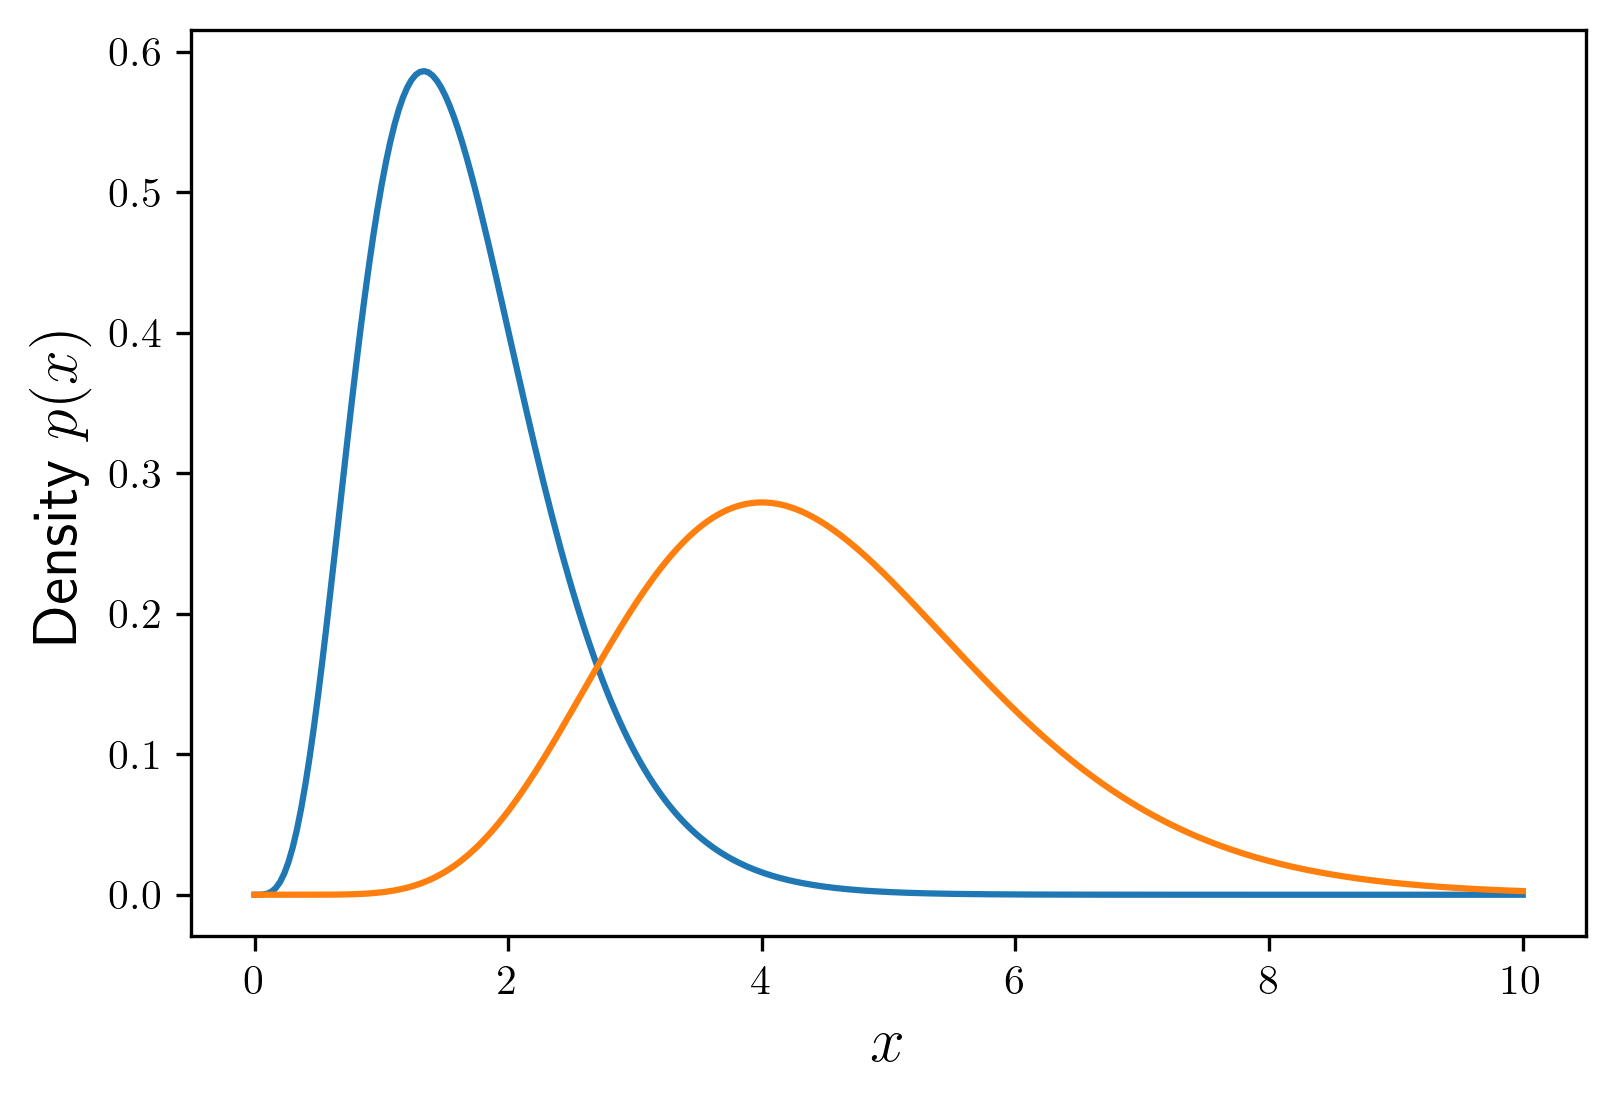
\includegraphics[width=0.8\textwidth]{./figures/stochastic_domination_pdf.png}
	\caption{Example of stochastic domination - PDFs}
	\label{fig:stochDomPDFs}
\end{figure}

Figure \ref{fig:stochDomPDFs} shows the probability density functions (PDFs) of two real random variables. In this example, the orange distribution stochastically dominates the blue distribution.

\begin{figure}[h]
	\centering
	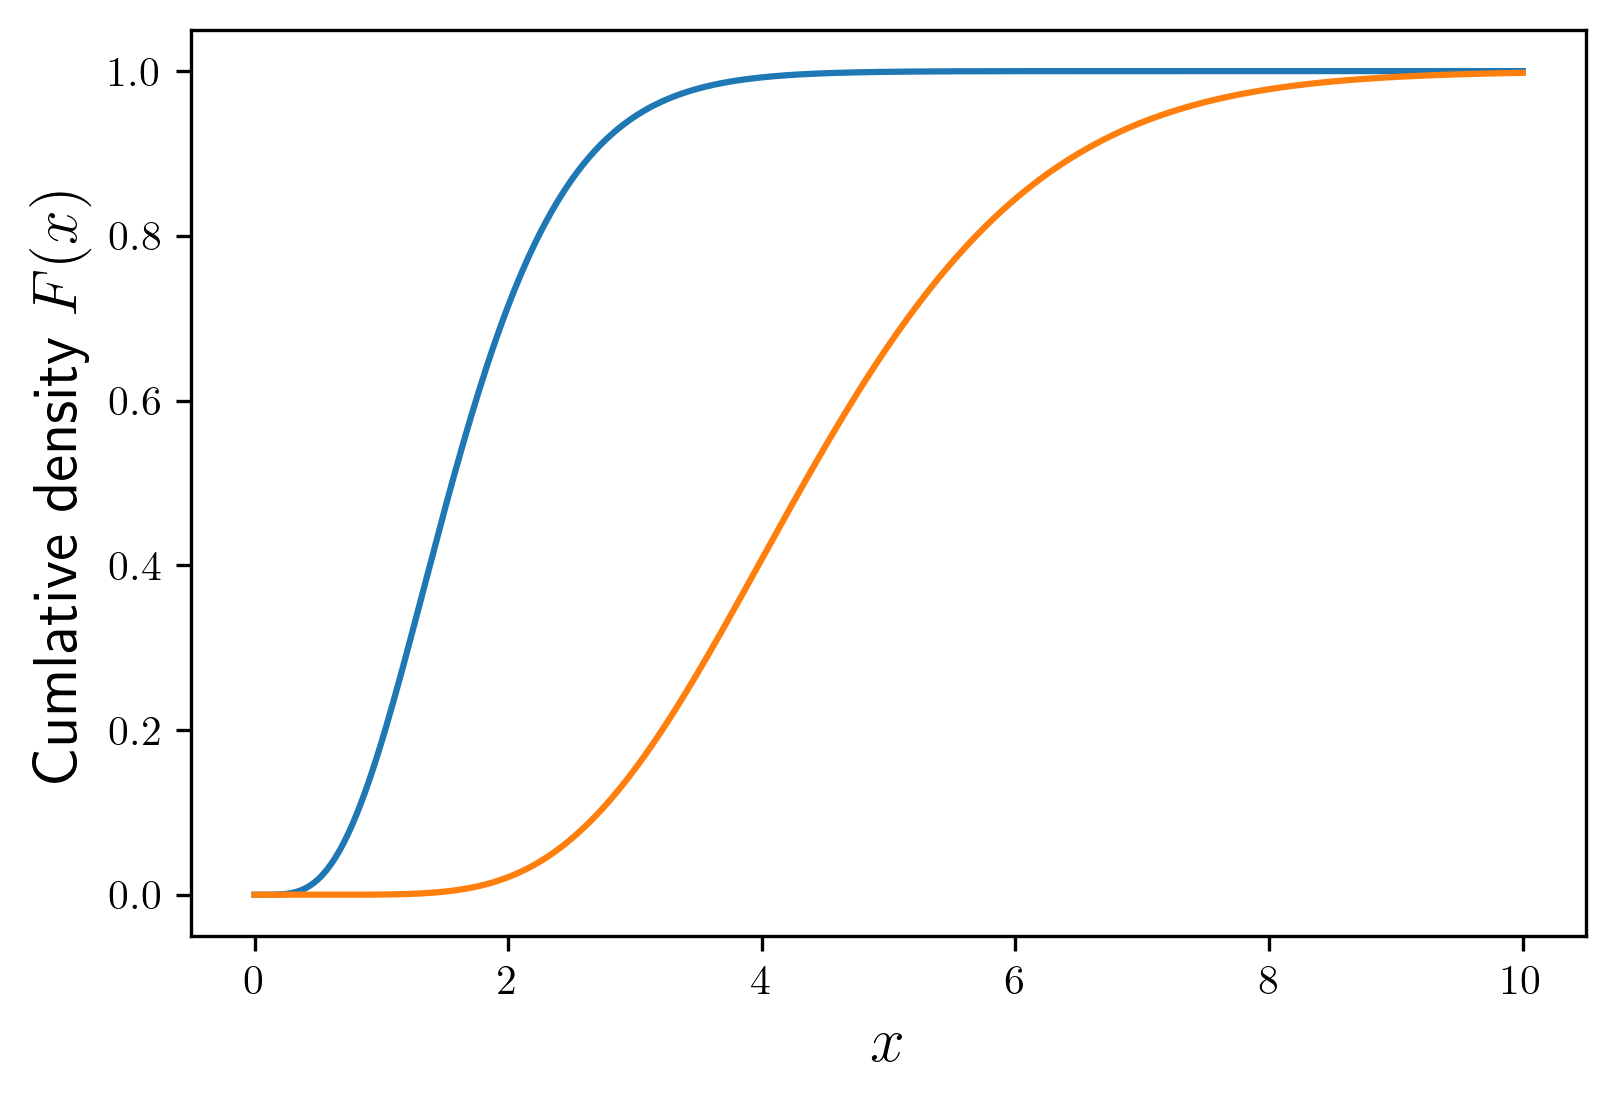
\includegraphics[width=0.8\textwidth]{./figures/stochastic_domination_cdf.png}
	\caption{Example of stochastic domination - CDFs}
	\label{fig:stochDomCDFs}
\end{figure}

Observe that $X \preceq Y$ if an only if $\mathbb{P}(Y \leq x) \leq \mathbb{P}(X \leq x)$. We recognise $\mathbb{P}(X \leq x)$ as the cumulative distribution function (CDF) of $X$. Hence, we verify this claim by computing the cumulative  distribution functions of the distributions in Figure \ref{fig:stochDomPDFs}, which are shown in Figure \ref{fig:stochDomCDFs}. Indeed, we see that the orange CDF is always below the blue CDF, hence the orange distribution does in fact dominate. % TODO: Reword, do we need this section?

For proofs in Chapters \ref{chapter:AsyncUpperBound} and \ref{chapter:SyncFlooding} we need to establish stochastic dominance between pairs of Binomial random variables and Poisson random variables. To do this we use a technique called coupling. First we introduce the definition of a coupling.

\begin{definition} % TODO: Check definition
	Coupling

	\noindent
	A  coupling of the real random variables $X$ and $Y$ is a joint random variable $(\tilde{X}, \tilde{Y})$ such that the marginal distribution of $\tilde{X}$ is the same as $X$, and the marginal distribution of $\tilde{Y}$ is the same as $Y$.
\end{definition}

% TODO: when allowed different samples spaces, interpreation

Now we present a theorem which links couplings to first-order stochastic domination.

\begin{theorem}\label{theorem:couplingDomination}
	The real random variable $X$ is stochastically dominated by the real random variable $Y$ if and only if there exists a coupling $(\tilde{X}, \tilde{Y})$ of $X$ and $Y$ such that
	$$
		\mathbb{P}(\tilde{Y} \geq \tilde{X}) = 1
	$$
\end{theorem}

\begin{proof}
	We prove the forwards implication. Suppose there exists a coupling $(\tilde{X}, \tilde{Y})$ of $X$ and $Y$ such that $\mathbb{P}(\tilde{Y} \geq \tilde{X}) = 1$. Then for all $x \in \mathbb{R}$
	\begin{align*}
		\mathbb{P}(X \geq x) &= \mathbb{P}(\tilde{X} \geq x) & \text{since } \tilde{X} \stackrel{d}{=} X \\
		&\leq \mathbb{P}(\tilde{Y} \geq x) & \text{since with probability 1, } \tilde{Y} \geq \tilde{X} \\
		&= \mathbb{P}(Y \geq x) & \text{since } \tilde{Y} \stackrel{d}{=} Y 
	\end{align*}

	We omit the proof for the reverse implication as we only use the forwards implication. For the proof of the reverse implication, see \cite{coupling}.
\end{proof}

% TODO, introduce equal in distribution in coupling definition

Using Theorem \ref{theorem:couplingDomination}, we can establish stochastic domination between random variables by finding a coupling. We first show this technique	for pairs of Poisson random variables

\begin{theorem}
	Let $0 < \lambda < \mu$. If $X \sim \text{Poisson}(\lambda)$ and $Y \sim \text{Poisson}(\mu)$ are independent random variables, then $X \preceq Y$. 
\end{theorem}

\begin{proof}
	Let $\tilde{X} \sim \text{Poisson}(\lambda)$, $\tilde{Z} \sim \text{Poisson}(\mu - \lambda)$ be independent random variables. Hence, we have that $\tilde{Y} := \tilde{X} + \tilde{Z} \sim \text{Poisson}(\mu)$. Note that since $\tilde{Z} \geq 0$, the value taken by $\tilde{Y}$ is always at least the value taken by $\tilde{X}$. Since we have found a coupling $(\tilde{X}, \tilde{Y})$ of $X$ and $Y$ where $\mathbb{P}(\tilde{Y} \geq \tilde{X}) = 1$, by Theorem \ref{theorem:couplingDomination}, $X \preceq Y$.
\end{proof}

Now we use coupling to establish first-order stochastic dominance between pairs of binomial random variables.

\begin{theorem}
	Let $X \sim \text{Binomial}(n_1, p)$ and $Y \sim \text{Binomial}(n_2, p)$ be independent random variables with $n_1 < n_2$. Then $X$ is stochastically dominated by $Y$.
\end{theorem}

\begin{proof}
	Let $X_1, \dots, X_{n_2}$ be an iid sequence of Bernoulli random variables where $\mathbb{P}(X_i = 1) = p$. We observe that $\tilde{X} := \sum_{i=1}^{n_1} X_i \sim \text{Binomial}(n_1, p)$ and $\tilde{Y} := \sum_{i=1}^{n_2} X_i \sim \text{Binomial}(n_2, p)$. Since $X_i \geq 0$ for all $i$, and $\tilde{Y} = \tilde{X} + X_{n_1 + 1} + \dots + X_{n_2}$, we have that $\tilde{X} \leq \tilde{Y}$. Hence, by Theorem \ref{theorem:couplingDomination}, $X \preceq Y$.
\end{proof}

% TODO: Move to own section, intro to networks??
\section{Introducing Dynamic Networks}

Here we formally define the Dynamic Network structure rumours will spread on.

\begin{definition}
	Dynamic Network

	\noindent
	A dynamic network is a sequence of graphs $\mathcal{G} = (G_t)_{t \in \mathbb{N}}$ indexed by an integer time $t$. All the graphs in the sequence have the same vertex set at each time step, but the edge set may vary, i.e.  $G_t = (V, E_t)$ where $E_t$ is some edge set on $V$.
\end{definition}

$G_t$ represents the topology of the network at the discrete time step $t$. However, asynchronous rumour spreading algorithms operate in continuous time, so we need to define the topology of the network at non-integer times. To represent the state of the network at any non-negative continuous time $\gamma \in \mathbb{R}_+$, we say that the current network topology $G_\gamma$ := $G_{\floor\gamma}$. Thus, for any time $\gamma \in [t, t + 1)$ the network topology is fixed to $G_t$. This corresponds to allowing the network topology change at integer time steps only.

% TODO: Segway

\begin{definition}
	Vertex degree at time $\gamma \in \mathbb{R}_+ $ 

	\noindent
	For a Dynamic Network $\mathcal{G}$ on a vertex set $V$, $d_v(\gamma)$ is the degree of a vertex $v \in V$ at time $\gamma$, i.e. the degree of $v$ in $G_\gamma$
\end{definition}


% TODO: DEFINITION OF ISOMORPHISM BETWEEN NETWORKSs

% TOD: definition of active and inactive edges in static rumour spreading section.

% TODO: Discuss implications for async rumour spreading - interpreting poission process as exponential clock, not interested in value of the process